\documentclass[a4paper]{article}
\usepackage[a4paper,margin=0mm]{geometry}
\usepackage{fontspec}
\usepackage{unicode-math}
\usepackage{tikz}
\usetikzlibrary{calc}
\usepackage[table]{xcolor}
\usepackage[absolute]{textpos}
\usepackage{enumitem}
\usepackage{array}
\usepackage{multirow}

\setmainfont{Libertinus Serif}
\setsansfont{Libertinus Sans}
\setmathfont{Libertinus Math}

\definecolor{accent}{HTML}{0F6A52}
\definecolor{badge}{HTML}{A9CFC2}
\definecolor{ink}{HTML}{2A2E30}

\setlength{\TPHorizModule}{1mm}
\setlength{\TPVertModule}{1mm}
\setlength{\parindent}{0pt}
\pagestyle{empty}
\binoppenalty=10000 \relpenalty=10000

\newcommand{\LCOL}{16mm}
\newcommand{\RCOL}{111mm}
\newcommand{\COLW}{83mm}

\newcommand{\topicheader}[2]{%
\begin{textblock*}{194mm}(16mm,10mm)
\begin{tikzpicture}
\node[fill=accent,text=white,font=\sffamily\bfseries\fontsize{13}{13}\selectfont,
      minimum width=9mm,minimum height=9mm,inner sep=0pt] at (4.5mm,-4.5mm) {#1};
\node[font=\sffamily\bfseries\fontsize{15}{16}\selectfont,text=ink,anchor=west] at (12mm,-4.5mm) {#2};
\end{tikzpicture}
\end{textblock*}
\begin{textblock*}{194mm}(16mm,22.5mm)

\begin{tikzpicture}
\fill[accent] (0,0) rectangle (194mm,0.5mm);
\end{tikzpicture}
\end{textblock*}
}

\newcommand{\pagefooter}[1]{%
\begin{textblock*}{194mm}(8mm,286.41mm)
  
\begin{tikzpicture}
    \fill[accent] (0,0) rectangle (194mm,0.6mm);
  \end{tikzpicture}
\end{textblock*}
\begin{textblock*}{63.59mm}(8mm,288.27mm)
  {\sffamily\bfseries\color{accent}\fontsize{13}{16}\selectfont SAT 1200+}
\end{textblock*}
\begin{textblock*}{10mm}(188mm,288.27mm)
  \centering{\sffamily\color{accent}\fontsize{14}{16}\selectfont #1}
\end{textblock*}
}

\newcommand{\colrule}[2]{%
\begin{textblock*}{1mm}(105mm,#1mm)
\begin{tikzpicture}
\draw[black!65,line width=0.5pt] (0,0) -- (0,#2mm);
\end{tikzpicture}
\end{textblock*}
}

% Page kicker: left = module line, right = question range
\newcommand{\pagekicker}[2]{%
\begin{textblock*}{194mm}(16mm,25.2mm)
{\sffamily\bfseries\fontsize{10.5}{12}\selectfont\color{accent}#1}\hfill{\sffamily\fontsize{10}{12}\selectfont\color{black!70}#2}
\end{textblock*}
}

\setlength{\fboxsep}{1.4pt}
\setlength{\fboxrule}{0.5pt}
\newcommand{\pnum}[1]{\fcolorbox{ink}{white}{\sffamily\bfseries\fontsize{8}{8}\selectfont #1}~}

% centered display line inside a stem
\newcommand{\dsp}[1]{\par\vspace{1.4mm}\centerline{#1}\vspace{1.8mm}}

% student-produced response box
\newcommand{\gridbox}{%
\par\vspace{3mm}\noindent

\begin{tikzpicture}
\node[anchor=south west,font=\sffamily\bfseries\fontsize{7.5}{9}\selectfont,text=accent,inner sep=0pt] at (0,0.3mm) {STUDENT-PRODUCED RESPONSE};
\draw[ink,line width=0.7pt] (0,-9.5mm) rectangle (40mm,-0.8mm);
\node[anchor=west,font=\sffamily\fontsize{7.5}{9}\selectfont,text=black!55,inner sep=0pt] at (43mm,-5.2mm) {Write your answer in the box.};
\end{tikzpicture}\par}

\arrayrulecolor{accent}
\setlength{\arrayrulewidth}{0.7pt}
\renewcommand{\arraystretch}{1.35}

\newcommand{\figwrap}[1]{\par\vspace{2.5mm}\centerline{{\arrayrulecolor{ink}\setlength{\arrayrulewidth}{0.5pt}\renewcommand{\arraystretch}{1.3}#1}}\vspace{0.5mm}}

\begin{document}

% ================= PAGE 1: Mock Test 8 -- instructions + geometry reference sheet =================
\topicheader{8}{Mock Test 8}
\pagefooter{1}
\mbox{}%

\newcommand{\cardhead}[1]{{\sffamily\bfseries\color{accent}\fontsize{11.5}{14}\selectfont #1}\par\vspace{0.6mm}%
{\color{accent}\rule{\linewidth}{0.5pt}}\par\vspace{1.6mm}}
\newcommand{\bul}{\item[\textcolor{accent}{\rule[0.2mm]{1.5mm}{1.5mm}}]}

\begin{textblock*}{194mm}(16mm,28mm)
{\sffamily\bfseries\color{accent}\fontsize{26}{28}\selectfont Mock Test 8\par}
\vspace{1mm}
{\sffamily\color{ink}\fontsize{11}{14}\selectfont Full-length digital SAT Math practice \;\textperiodcentered\; 2 modules $\times$ 22 questions $\times$ 35 minutes\par}
\end{textblock*}

\begin{textblock*}{\COLW}(\LCOL,53mm)
{\fontsize{9.4}{12.2}\selectfont
\cardhead{How this test works}
\renewcommand{\arraystretch}{1.3}\setlength{\tabcolsep}{4pt}
\noindent\begin{tabular}{|>{\raggedright\arraybackslash}p{20mm}|>{\centering\arraybackslash}p{15mm}|>{\centering\arraybackslash}p{13mm}|>{\centering\arraybackslash}p{19mm}|}
\hline
\rowcolor{badge!55}\textbf{Module} & \textbf{Questions} & \textbf{Time} & \textbf{Calculator}\\\hline
Module 1 & 22 & 35 min & allowed\\\hline
Module 2 & 22 & 35 min & allowed\\\hline
\end{tabular}\par\vspace{2.2mm}
\begin{itemize}[leftmargin=5mm,itemsep=1.2mm,topsep=0mm,parsep=0mm]
\bul Time each module separately: 35 minutes, not a minute more. Rest for 5--10 minutes between the two modules.
\bul Use a calculator (the built-in Desmos graphing calculator or any approved calculator) on both modules.
\bul Module 1 is a standard mix of easy, medium and hard questions. Module 2 is the \emph{harder route} you reach by doing well on Module 1.
\bul Answer every question. There is no penalty for a wrong answer.
\bul Unless a problem says otherwise, all numbers are real, a function's domain is every real number for which it is defined, and figures are not necessarily drawn to scale.
\bul Do not look at any answers while you work. When you finish both modules, score yourself with the \textbf{Answer Sheets} section at the end of this book.
\end{itemize}
}
\end{textblock*}

\begin{textblock*}{\COLW}(\RCOL,53mm)
{\fontsize{9.4}{12.2}\selectfont
\cardhead{Student-produced responses (grid-ins)}
Some questions have no answer choices. Work out the answer and write it in the answer box (on the real test you type it in).
\begin{itemize}[leftmargin=5mm,itemsep=1.2mm,topsep=1.6mm,parsep=0mm]
\bul You may give an integer, a decimal, or a fraction. For one answer, $9/2$ and $4.5$ are both correct.
\bul Never enter a mixed number: write $7/2$ or $3.5$, not $3\,1/2$ (it would be read as $31/2$).
\bul Do not enter symbols or units such as \$, \%, or $\pi$. Enter the number only.
\bul An answer may use at most 5 characters (6 if it is negative), counting the slash and the decimal point.
\bul If an answer is a repeating decimal, enter it as a fraction such as $2/3$, or fill all the digits that fit: $0.6666$ or $0.6667$.
\bul If you find more than one correct answer, enter only one of them.
\end{itemize}
\vspace{1.2mm}
\noindent\fcolorbox{accent}{badge!25}{\parbox{\dimexpr\linewidth-2\fboxsep-2\fboxrule}{\centering\sffamily\fontsize{8.5}{11}\selectfont
\textbf{Example.} Answer $4\tfrac12$ \;$\rightarrow$\; enter \textbf{9/2} or \textbf{4.5}\par}}
\par\vspace{3mm}
\noindent{\sffamily\bfseries\color{accent}Pacing.}\ Q1--15: about 18 min. Q16--22: about 17 min. Keep the last 2--3 min for flagged questions and every blank grid-in (a blank is a guaranteed zero).
}
\end{textblock*}

% ---- Geometry reference sheet (full width card) ----
\begin{textblock*}{178mm}(16mm,156mm)
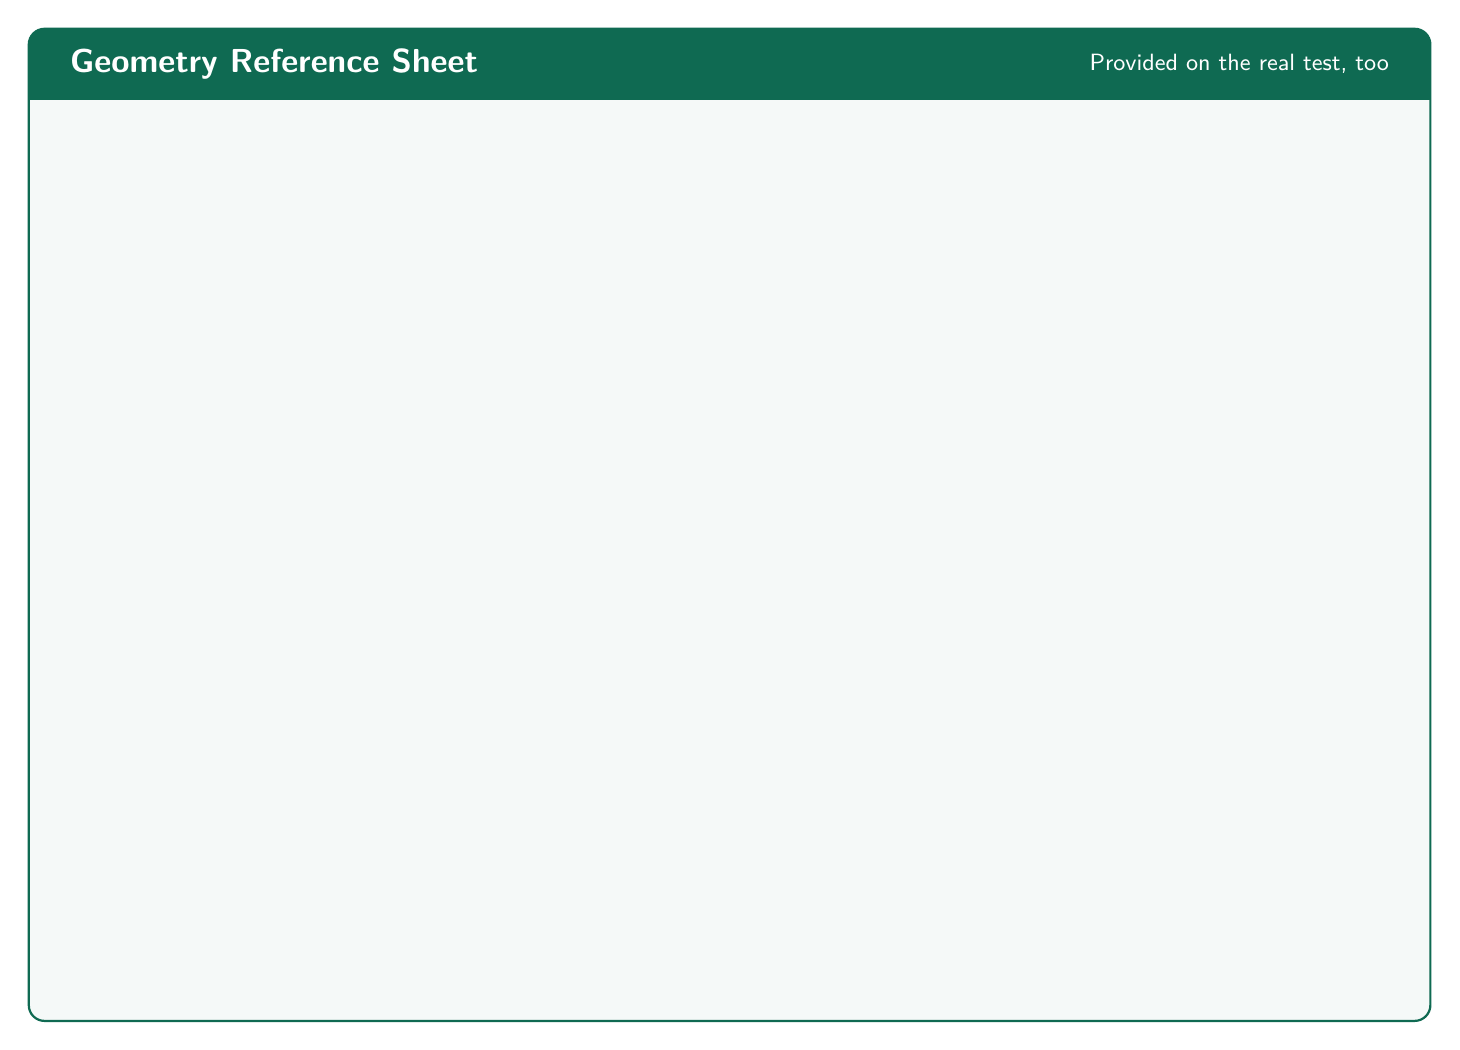
\begin{tikzpicture}
\draw[accent,line width=0.8pt,rounded corners=2mm,fill=badge!12] (0,0) rectangle (178mm,-126mm);
\fill[accent,rounded corners=2mm] (0,0) rectangle (178mm,-9mm);
\fill[accent] (0,-5mm) rectangle (178mm,-9mm);
\node[anchor=west,text=white,font=\sffamily\bfseries\fontsize{12}{14}\selectfont] at (4mm,-4.5mm) {Geometry Reference Sheet};
\node[anchor=east,text=white,font=\sffamily\fontsize{8.5}{10}\selectfont] at (174mm,-4.5mm) {Provided on the real test, too};
\end{tikzpicture}
\end{textblock*}

\newcommand{\refcell}[3]{\begin{textblock*}{42mm}(#1mm,#2mm)\begin{minipage}[t][36mm][t]{42mm}\centering #3\end{minipage}\end{textblock*}}
\newcommand{\refin}[2]{\parbox[b][26mm][b]{42mm}{\centering #1}\par\vspace{1.6mm}{\fontsize{9.6}{11.5}\selectfont #2}}
\tikzset{rf/.style={ink,line width=0.65pt},lb/.style={font=\fontsize{8.5}{9.5}\selectfont,inner sep=1.2pt}}

% ---------- row 1
\refcell{18}{167}{\refin{\begin{tikzpicture}[scale=1.25]
\draw[rf] (0,0) circle (9mm); \draw[rf] (0,0)--(9mm,0); \fill[ink] (0,0) circle (0.7pt);
\node[lb,above] at (4.5mm,0) {$r$};
\end{tikzpicture}}{Circle\\$A=\pi r^{2}$,\; $C=2\pi r$}}
\refcell{62}{167}{\refin{\begin{tikzpicture}[scale=1.25]
\draw[rf] (0,0) rectangle (22mm,12mm);
\node[lb,below] at (11mm,0) {$\ell$}; \node[lb,right] at (22mm,6mm) {$w$};
\end{tikzpicture}}{Rectangle\\$A=\ell w$}}
\refcell{106}{167}{\refin{\begin{tikzpicture}[scale=1.25]
\draw[rf] (0,0)--(22mm,0)--(7mm,13mm)--cycle;
\draw[rf,dashed] (7mm,0)--(7mm,13mm);
\draw[rf] (7mm,0)++(0,1.8mm)--++(1.8mm,0)--++(0,-1.8mm);
\node[lb,below] at (11mm,0) {$b$}; \node[lb,left] at (7mm,6.5mm) {$h$};
\end{tikzpicture}}{Triangle\\$A=\tfrac12 bh$}}
\refcell{150}{167}{\refin{\begin{tikzpicture}[scale=1.25]
\draw[rf] (0,0)--(18mm,0)--(0,12mm)--cycle;
\draw[rf] (0,1.8mm)--(1.8mm,1.8mm)--(1.8mm,0);
\node[lb,below] at (9mm,0) {$a$}; \node[lb,left] at (0,6mm) {$b$}; \node[lb,above right] at (9mm,6mm) {$c$};
\end{tikzpicture}}{Right triangle\\$c^{2}=a^{2}+b^{2}$}}

% ---------- row 2
\refcell{18}{204}{\refin{\begin{tikzpicture}[scale=1.25]
\draw[rf] (0,0)--(19.053mm,0)--(0,11mm)--cycle;
\draw[rf] (0,1.8mm)--(1.8mm,1.8mm)--(1.8mm,0);
\node[lb,below] at (9.5mm,0) {$x\sqrt3$}; \node[lb,left] at (0,5.5mm) {$x$}; \node[lb,above right] at (9.5mm,5.5mm) {$2x$};
\node[lb] at (14.6mm,1.9mm) {\fontsize{6.5}{7}\selectfont$30^\circ$}; \node[lb] at (3.2mm,8.2mm) {\fontsize{6.5}{7}\selectfont$60^\circ$};
\end{tikzpicture}}{$30^\circ$--$60^\circ$--$90^\circ$ triangle}}
\refcell{62}{204}{\refin{\begin{tikzpicture}[scale=1.25]
\draw[rf] (0,0)--(10mm,0)--(0,10mm)--cycle;
\draw[rf] (0,1.8mm)--(1.8mm,1.8mm)--(1.8mm,0);
\node[lb,below] at (5mm,0) {$s$}; \node[lb,left] at (0,5mm) {$s$}; \node[lb,above right] at (5mm,5mm) {$s\sqrt2$};
\end{tikzpicture}}{$45^\circ$--$45^\circ$--$90^\circ$ triangle}}
\refcell{106}{204}{\refin{\begin{tikzpicture}[scale=1.2]
\draw[rf] (0,0) rectangle (16mm,9mm);
\draw[rf] (16mm,9mm)--(22mm,13mm)--(6mm,13mm)--(0,9mm);
\draw[rf] (16mm,0)--(22mm,4mm)--(22mm,13mm);
\draw[rf,dashed] (6mm,13mm)--(6mm,4mm)--(22mm,4mm); \draw[rf,dashed] (0,0)--(6mm,4mm);
\node[lb,below] at (8mm,0) {$\ell$}; \node[lb,right] at (22mm,8.5mm) {$h$}; \node[lb,below right] at (19mm,2mm) {$w$};
\end{tikzpicture}}{Rectangular solid\\$V=\ell wh$}}
\refcell{150}{204}{\refin{\begin{tikzpicture}[scale=1.2]
\draw[rf] (0,2.2mm) ellipse (7mm and 2.2mm);
\draw[rf] (-7mm,2.2mm)--(-7mm,14mm); \draw[rf] (7mm,2.2mm)--(7mm,14mm);
\draw[rf] (0,14mm) ellipse (7mm and 2.2mm);
\draw[rf,dashed] (0,14mm)--(7mm,14mm); \fill[ink] (0,14mm) circle (0.6pt);
\node[lb,above] at (3.5mm,14mm) {$r$}; \node[lb,right] at (7mm,8mm) {$h$};
\end{tikzpicture}}{Right circular cylinder\\$V=\pi r^{2}h$}}

% ---------- row 3
\refcell{18}{241}{\refin{\begin{tikzpicture}[scale=1.15]
\draw[rf] (0,0) circle (10mm);
\draw[rf] (-10mm,0) arc (180:360:10mm and 2.8mm); \draw[rf,dashed] (-10mm,0) arc (180:0:10mm and 2.8mm);
\draw[rf] (0,0)--(10mm,0); \fill[ink] (0,0) circle (0.7pt); \node[lb,above] at (5mm,0) {$r$};
\end{tikzpicture}}{Sphere\\$V=\tfrac43\pi r^{3}$}}
\refcell{62}{241}{\refin{\begin{tikzpicture}[scale=1.2]
\draw[rf] (0,2.2mm) ellipse (7mm and 2.2mm);
\draw[rf] (-7mm,2.2mm)--(0,16mm)--(7mm,2.2mm);
\draw[rf,dashed] (0,16mm)--(0,2.2mm); \draw[rf,dashed] (0,2.2mm)--(7mm,2.2mm);
\fill[ink] (0,2.2mm) circle (0.6pt);
\node[lb,left] at (0,9.5mm) {$h$}; \node[lb,above] at (3.5mm,2.2mm) {$r$};
\end{tikzpicture}}{Right circular cone\\$V=\tfrac13\pi r^{2}h$}}
\refcell{106}{241}{\refin{\begin{tikzpicture}[scale=1.2]
\draw[rf] (0,0)--(16mm,0)--(22mm,4mm); \draw[rf] (0,0)--(10mm,15mm)--(16mm,0); \draw[rf] (10mm,15mm)--(22mm,4mm);
\draw[rf,dashed] (0,0)--(6mm,4mm)--(22mm,4mm); \draw[rf,dashed] (6mm,4mm)--(10mm,15mm);
\node[lb,below] at (8mm,0) {$\ell$}; \node[lb,below right] at (19mm,2mm) {$w$}; \node[lb,left] at (10mm,9.5mm) {$h$};
\end{tikzpicture}}{Rectangular pyramid\\$V=\tfrac13\ell wh$}}
\begin{textblock*}{40mm}(151mm,247mm)
{\fontsize{9.2}{12}\selectfont\raggedright
\textcolor{accent}{\rule[0.3mm]{1.6mm}{1.6mm}}\; A circle has 360 degrees of arc.\par\vspace{1.2mm}
\textcolor{accent}{\rule[0.3mm]{1.6mm}{1.6mm}}\; The angles of a triangle add up to 180 degrees.\par\vspace{1.2mm}
\textcolor{accent}{\rule[0.3mm]{1.6mm}{1.6mm}}\; $r$ radius, $\ell$ length, $w$ width, $b$ base, $h$ height.\par}
\end{textblock*}

\clearpage

% ===== Module 1, page 1 =====
\topicheader{8}{Mock Test 8}
\pagefooter{2}
\colrule{34}{236}
\mbox{}%
\pagekicker{Mock 8 \textperiodcentered{} Module 1 \textperiodcentered{} 22 questions \textperiodcentered{} 35 minutes}{Questions 1--8}
\begin{textblock*}{\COLW}(\LCOL,34mm)
{\fontsize{10.4}{13.4}\selectfont
\parbox[t][233mm][t]{\COLW}{%
\noindent\pnum{1} A construction crew has already laid 30 meters of drainage pipe. It lays 15 more meters each day, and the job requires a total of 150 meters. How many more days will the crew need to finish laying the pipe?\par\vspace{2.2mm}
\hspace*{7mm}(A)\ $10$\\[1.8mm]
\hspace*{7mm}(B)\ $8$\\[1.8mm]
\hspace*{7mm}(C)\ $12$\\[1.8mm]
\hspace*{7mm}(D)\ $120$
\vfill

\noindent\pnum{2} Which of the following is equivalent to $\sqrt{50}$?\par\vspace{2.2mm}
\hspace*{7mm}(A)\ $5\sqrt{2}$\\[1.8mm]
\hspace*{7mm}(B)\ $25\sqrt{2}$\\[1.8mm]
\hspace*{7mm}(C)\ $10\sqrt{5}$\\[1.8mm]
\hspace*{7mm}(D)\ $5\sqrt{10}$
\vfill

\noindent\pnum{3} In a school election, 126 students voted for Ortiz. That was 30\% of all the votes cast. How many votes were cast in the election?\gridbox
\vfill

\noindent\pnum{4} At the same time of day, a vertical pole 2 meters tall casts a shadow 3 meters long, and a tree casts a shadow 15 meters long. What is the height, in meters, of the tree?\par\vspace{2.2mm}
\hspace*{7mm}(A)\ $22.5$\\[1.8mm]
\hspace*{7mm}(B)\ $14$\\[1.8mm]
\hspace*{7mm}(C)\ $5$\\[1.8mm]
\hspace*{7mm}(D)\ $10$
\vfill}}
\end{textblock*}
\begin{textblock*}{\COLW}(\RCOL,34mm)
{\fontsize{10.4}{13.4}\selectfont
\parbox[t][233mm][t]{\COLW}{%
\noindent\pnum{5} If $3(x+4)=2x+19$, what is the value of $x$?\par\vspace{2.2mm}
\hspace*{7mm}(A)\ $15$\\[1.8mm]
\hspace*{7mm}(B)\ $31$\\[1.8mm]
\hspace*{7mm}(C)\ $7$\\[1.8mm]
\hspace*{7mm}(D)\ $1.4$
\vfill

\noindent\pnum{6} What is the sum of the solutions of the equation $(x-4)(x+9)=0$?\par\vspace{2.2mm}
\hspace*{7mm}(A)\ $5$\\[1.8mm]
\hspace*{7mm}(B)\ $-5$\\[1.8mm]
\hspace*{7mm}(C)\ $13$\\[1.8mm]
\hspace*{7mm}(D)\ $-13$
\vfill

\noindent\pnum{7} Hira's training plan has her run 12 miles in week 1. Each week she increases her weekly distance by 2.5 miles. How many miles will she run in week 7?\gridbox
\vfill

\noindent\pnum{8} For $x>0$, which of the following is equivalent to $\dfrac{15x^{7}}{3x^{4}}$?\par\vspace{2.2mm}
\hspace*{7mm}(A)\ $5x^{3}$\\[1.8mm]
\hspace*{7mm}(B)\ $12x^{3}$\\[1.8mm]
\hspace*{7mm}(C)\ $5x^{7/4}$\\[1.8mm]
\hspace*{7mm}(D)\ $5x^{11}$
\vfill}}
\end{textblock*}
\clearpage

% ===== Module 1, page 2 =====
\topicheader{8}{Mock Test 8}
\pagefooter{3}
\colrule{34}{236}
\mbox{}%
\pagekicker{Mock 8 \textperiodcentered{} Module 1 \textperiodcentered{} 22 questions \textperiodcentered{} 35 minutes}{Questions 9--16}
\begin{textblock*}{\COLW}(\LCOL,34mm)
{\fontsize{10.4}{13.4}\selectfont
\parbox[t][233mm][t]{\COLW}{%
\noindent\pnum{9} A coach randomly selects 2 of her 12 players to demonstrate a drill. Five of the 12 players are seniors. What is the probability that both of the selected players are seniors?\par\vspace{2.2mm}
\hspace*{7mm}(A)\ $\dfrac{25}{144}$\\[1.8mm]
\hspace*{7mm}(B)\ $\dfrac{5}{66}$\\[1.8mm]
\hspace*{7mm}(C)\ $\dfrac{5}{33}$\\[1.8mm]
\hspace*{7mm}(D)\ $\dfrac{5}{6}$
\vfill

\noindent\pnum{10} A protein bar has 20 grams of protein and 250 calories. A protein shake has 30 grams of protein and 180 calories. An athlete's meal plan uses only bars and shakes and must provide exactly 130 grams of protein and exactly 1,040 calories. How many shakes are in the plan?\gridbox
\vfill

\noindent\pnum{11} For $x>0$, which of the following is equivalent to $\sqrt{18x^{5}}$?\par\vspace{2.2mm}
\hspace*{7mm}(A)\ $9x^{2}\sqrt{2x}$\\[1.8mm]
\hspace*{7mm}(B)\ $3x^{3}\sqrt{2}$\\[1.8mm]
\hspace*{7mm}(C)\ $3x^{2}\sqrt{2}$\\[1.8mm]
\hspace*{7mm}(D)\ $3x^{2}\sqrt{2x}$
\vfill

\noindent\pnum{12} In the $xy$-plane, point $M$ is the midpoint of the segment with endpoints $A(-2,1)$ and $B(6,7)$. What is the distance from the origin to $M$?\par\vspace{2.2mm}
\hspace*{7mm}(A)\ $2\sqrt{5}$\\[1.8mm]
\hspace*{7mm}(B)\ $4\sqrt{5}$\\[1.8mm]
\hspace*{7mm}(C)\ $10$\\[1.8mm]
\hspace*{7mm}(D)\ $2\sqrt{13}$
\vfill}}
\end{textblock*}
\begin{textblock*}{\COLW}(\RCOL,34mm)
{\fontsize{10.4}{13.4}\selectfont
\parbox[t][233mm][t]{\COLW}{%
\noindent\pnum{13} During a conditioning session that lasts exactly 60 minutes, Kofi runs for part of the time and rows for the rest. Running burns 11 calories per minute and rowing burns 8 calories per minute. He wants to burn at least 600 calories. What is the least number of minutes he must spend running?\par\vspace{2.2mm}
\hspace*{7mm}(A)\ $55$\\[1.8mm]
\hspace*{7mm}(B)\ $40$\\[1.8mm]
\hspace*{7mm}(C)\ $11$\\[1.8mm]
\hspace*{7mm}(D)\ $75$
\vfill

\noindent\pnum{14} A \$15,000 piece of equipment loses 20\% of its value each year, with each year's loss based on its value at the start of that year. What is the value of the equipment, in dollars, 3 years after it was purchased?\gridbox
\vfill

\noindent\pnum{15} A truck is loaded with crates of concrete blocks and steel beams. Each crate weighs 2.4 tonnes and each beam weighs 1.5 tonnes. The equation $2.4c+1.5s=18$ represents loads that total exactly 18 tonnes, where $c$ is the number of crates and $s$ is the number of beams. According to the equation, if the truck keeps carrying exactly 18 tonnes, loading one more crate means loading how many fewer beams?\par\vspace{2.2mm}
\hspace*{7mm}(A)\ $0.625$\\[1.8mm]
\hspace*{7mm}(B)\ $2.4$\\[1.8mm]
\hspace*{7mm}(C)\ $12$\\[1.8mm]
\hspace*{7mm}(D)\ $1.6$
\vfill

\noindent\pnum{16} For $a>0$ and $b>0$, which of the following is equivalent to $\dfrac{(2a^{-1}b^{2})^{3}}{4a^{-5}b}$?\par\vspace{2.2mm}
\hspace*{7mm}(A)\ $2a^{-8}b^{5}$\\[1.8mm]
\hspace*{7mm}(B)\ $8a^{2}b^{5}$\\[1.8mm]
\hspace*{7mm}(C)\ $2a^{2}b^{5}$\\[1.8mm]
\hspace*{7mm}(D)\ $2a^{-2}b^{5}$
\vfill}}
\end{textblock*}
\clearpage

% ===== Module 1, page 3 =====
\topicheader{8}{Mock Test 8}
\pagefooter{4}
\colrule{34}{236}
\mbox{}%
\pagekicker{Mock 8 \textperiodcentered{} Module 1 \textperiodcentered{} 22 questions \textperiodcentered{} 35 minutes}{Questions 17--22}
\begin{textblock*}{\COLW}(\LCOL,34mm)
{\fontsize{10.4}{13.4}\selectfont
\parbox[t][233mm][t]{\COLW}{%
\noindent\pnum{17} The expression $(2x-1)(x+3)(x-4)$ is expanded and written in the form $px^{3}+qx^{2}+rx+s$, where $p$, $q$, $r$, and $s$ are constants. What is the value of $p+q+r+s$?\gridbox
\vfill

\noindent\pnum{18} The table shows the number of votes cast for each candidate in a school election, by the grade level of the voter. One of the votes cast for Walsh is selected at random. What is the probability that this vote came from a 10th grader?\figwrap{\begin{tabular}{|l|c|c|c|}
\hline
 & Grade 9 & Grade 10 & Grade 11\\\hline
Reyes & 48 & 30 & 42\\\hline
Walsh & 36 & 45 & 39\\\hline
Ng & 16 & 25 & 19\\\hline
\end{tabular}}\par\vspace{2.2mm}
\hspace*{7mm}(A)\ $\dfrac{3}{8}$\\[1.8mm]
\hspace*{7mm}(B)\ $\dfrac{9}{20}$\\[1.8mm]
\hspace*{7mm}(C)\ $\dfrac{3}{20}$\\[1.8mm]
\hspace*{7mm}(D)\ $\dfrac{2}{5}$
\vfill

\noindent\pnum{19} A navigation log shows an airplane's distance $d$, in nautical miles, from its departure airport $t$ hours after 10:00 a.m. At $t=0.5$ the distance was 120, and at $t=2$ it was 450. Assume $d$ is a linear function of $t$. What was the distance, in nautical miles, at $t=3.5$?\par\vspace{2.2mm}
\hspace*{7mm}(A)\ $840$\\[1.8mm]
\hspace*{7mm}(B)\ $780$\\[1.8mm]
\hspace*{7mm}(C)\ $787.5$\\[1.8mm]
\hspace*{7mm}(D)\ $810$
\vfill}}
\end{textblock*}
\begin{textblock*}{\COLW}(\RCOL,34mm)
{\fontsize{10.4}{13.4}\selectfont
\parbox[t][233mm][t]{\COLW}{%
\noindent\pnum{20} A bond fund is worth \$25,000 today and loses 18\% of its value each year. Which of the following expressions gives the value of the fund, in dollars, $m$ months from today?\par\vspace{2.2mm}
\hspace*{7mm}(A)\ $25{,}000(0.82)^{12m}$\\[1.8mm]
\hspace*{7mm}(B)\ $25{,}000(0.985)^{m}$\\[1.8mm]
\hspace*{7mm}(C)\ $25{,}000(0.18)^{m/12}$\\[1.8mm]
\hspace*{7mm}(D)\ $25{,}000(0.82)^{m/12}$
\vfill

\noindent\pnum{21} If $\dfrac{5x+y}{2x-y}=4$ and $y\ne0$, what is the value of $\dfrac{x}{y}$?\gridbox
\vfill

\noindent\pnum{22} In the $xy$-plane, the graph of $x^{2}+y^{2}-6x+8y=0$ is a circle that passes through the origin. Which of the following is an equation of the line tangent to the circle at the origin?\par\vspace{2.2mm}
\hspace*{7mm}(A)\ $y=-\dfrac{4}{3}x$\\[1.8mm]
\hspace*{7mm}(B)\ $y=\dfrac{4}{3}x$\\[1.8mm]
\hspace*{7mm}(C)\ $y=\dfrac{3}{4}x$\\[1.8mm]
\hspace*{7mm}(D)\ $y=-\dfrac{3}{4}x$
\vfill}}
\end{textblock*}
\clearpage

% ===== Module 2, page 1 =====
\topicheader{8}{Mock Test 8}
\pagefooter{5}
\colrule{34}{236}
\mbox{}%
\pagekicker{Mock 8 \textperiodcentered{} Module 2 \textperiodcentered{} 22 questions \textperiodcentered{} 35 minutes}{Questions 1--8}
\begin{textblock*}{\COLW}(\LCOL,34mm)
{\fontsize{10.4}{13.4}\selectfont
\parbox[t][233mm][t]{\COLW}{%
\noindent\pnum{1} The sum of three numbers is 90. The second number is twice the first number, and the third number is 3 times the first number. What is the greatest of the three numbers?\par\vspace{2.2mm}
\hspace*{7mm}(A)\ $15$\\[1.8mm]
\hspace*{7mm}(B)\ $30$\\[1.8mm]
\hspace*{7mm}(C)\ $60$\\[1.8mm]
\hspace*{7mm}(D)\ $45$
\vfill

\noindent\pnum{2} The function $p$ is defined by $p(x)=x^{3}-2x$. What is the value of $p(-2)$?\par\vspace{2.2mm}
\hspace*{7mm}(A)\ $-4$\\[1.8mm]
\hspace*{7mm}(B)\ $4$\\[1.8mm]
\hspace*{7mm}(C)\ $12$\\[1.8mm]
\hspace*{7mm}(D)\ $-12$
\vfill

\noindent\pnum{3} For $x\ne-\frac{1}{2}$, which of the following is equivalent to $\dfrac{6x^{2}-5x-4}{2x+1}$?\par\vspace{2.2mm}
\hspace*{7mm}(A)\ $3x+4$\\[1.8mm]
\hspace*{7mm}(B)\ $-2x-4$\\[1.8mm]
\hspace*{7mm}(C)\ $3x-4$\\[1.8mm]
\hspace*{7mm}(D)\ $3x-1$
\vfill

\noindent\pnum{4} During a 4.5-hour cycling race, a rider's nutrition plan calls for 1.1 grams of carbohydrate per kilogram of body weight per hour. The rider weighs 72 kilograms, and each energy gel contains 24 grams of carbohydrate. What is the least number of gels the rider must take to meet the plan?\gridbox
\vfill}}
\end{textblock*}
\begin{textblock*}{\COLW}(\RCOL,34mm)
{\fontsize{10.4}{13.4}\selectfont
\parbox[t][233mm][t]{\COLW}{%
\noindent\pnum{5} A plane's airspeed in still air is 270 miles per hour. Flying a straight route with a steady tailwind, the plane takes 4 hours to go from city $P$ to city $Q$. Flying back along the same route against the same steady wind, it takes 5 hours. How many miles is it from $P$ to $Q$?\par\vspace{2.2mm}
\hspace*{7mm}(A)\ $1{,}080$\\[1.8mm]
\hspace*{7mm}(B)\ $1{,}200$\\[1.8mm]
\hspace*{7mm}(C)\ $1{,}350$\\[1.8mm]
\hspace*{7mm}(D)\ $30$
\vfill

\noindent\pnum{6} After takeoff, an airplane climbs along a straight path that makes an angle $\theta$ with level ground, where $\sin\theta=0.28$. After the plane has flown 7,500 feet along this path, how many feet of horizontal ground distance has it covered?\par\vspace{2.2mm}
\hspace*{7mm}(A)\ $2{,}100$\\[1.8mm]
\hspace*{7mm}(B)\ $5{,}400$\\[1.8mm]
\hspace*{7mm}(C)\ $7{,}200$\\[1.8mm]
\hspace*{7mm}(D)\ $7{,}500$
\vfill

\noindent\pnum{7} The opening under a stone arch bridge is modeled by $h=20-0.05x^{2}$, where $x$ is the horizontal distance, in meters, from the center line of the opening and $h$ is the height, in meters, above the water. A barge must pass through the opening with at least 15 meters of clearance above the water along its entire width. If the barge is centered under the arch, what is the greatest possible width, in meters, of the barge?\par\vspace{2.2mm}
\hspace*{7mm}(A)\ $10$\\[1.8mm]
\hspace*{7mm}(B)\ $20$\\[1.8mm]
\hspace*{7mm}(C)\ $40$\\[1.8mm]
\hspace*{7mm}(D)\ $100$
\vfill

\noindent\pnum{8} In the $xy$-plane, the perpendicular bisector of the segment with endpoints $A(2,-3)$ and $B(10,9)$ crosses the $y$-axis at the point $(0,k)$. What is the value of $k$?\gridbox
\vfill}}
\end{textblock*}
\clearpage

% ===== Module 2, page 2 =====
\topicheader{8}{Mock Test 8}
\pagefooter{6}
\colrule{34}{236}
\mbox{}%
\pagekicker{Mock 8 \textperiodcentered{} Module 2 \textperiodcentered{} 22 questions \textperiodcentered{} 35 minutes}{Questions 9--16}
\begin{textblock*}{\COLW}(\LCOL,34mm)
{\fontsize{10.4}{13.4}\selectfont
\parbox[t][233mm][t]{\COLW}{%
\noindent\pnum{9} The function $f$ is defined by $f(x)=2x^{2}-12x+7$. Which of the following is an equivalent form of $f$ in which the minimum value of $f$ appears as a constant or coefficient?\par\vspace{2.2mm}
\hspace*{7mm}(A)\ $2(x-3)^{2}-11$\\[1.8mm]
\hspace*{7mm}(B)\ $2x^{2}-12x+7$\\[1.8mm]
\hspace*{7mm}(C)\ $2x(x-6)+7$\\[1.8mm]
\hspace*{7mm}(D)\ $2(x^{2}-6x)+7$
\vfill

\noindent\pnum{10} In the $xy$-plane, a line passes through the points $(2k,\,k+3)$ and $(k+3,\,2k)$, where $k\ne3$. What is the slope of the line?\par\vspace{2.2mm}
\hspace*{7mm}(A)\ $1$\\[1.8mm]
\hspace*{7mm}(B)\ $\dfrac{2k}{k+3}$\\[1.8mm]
\hspace*{7mm}(C)\ $k-3$\\[1.8mm]
\hspace*{7mm}(D)\ $-1$
\vfill

\noindent\pnum{11} A mobile crane's lifting capacity decreases at a constant rate as the boom reach increases. At a reach of 10 meters the crane can lift 20 tonnes, and at a reach of 26 meters it can lift 12 tonnes. At what reach, in meters, can the crane lift exactly 15 tonnes?\par\vspace{2.2mm}
\hspace*{7mm}(A)\ $16$\\[1.8mm]
\hspace*{7mm}(B)\ $18$\\[1.8mm]
\hspace*{7mm}(C)\ $20$\\[1.8mm]
\hspace*{7mm}(D)\ $25$
\vfill

\noindent\pnum{12} The line $y=2x-4$ is reflected across the $y$-axis, and the resulting line is then translated 3 units up. Which of the following is an equation of the final line?\par\vspace{2.2mm}
\hspace*{7mm}(A)\ $y=-2x+7$\\[1.8mm]
\hspace*{7mm}(B)\ $y=-2x-1$\\[1.8mm]
\hspace*{7mm}(C)\ $y=2x-1$\\[1.8mm]
\hspace*{7mm}(D)\ $y=-2x-7$
\vfill}}
\end{textblock*}
\begin{textblock*}{\COLW}(\RCOL,34mm)
{\fontsize{10.4}{13.4}\selectfont
\parbox[t][233mm][t]{\COLW}{%
\noindent\pnum{13} In the $xy$-plane, the line $y=-\frac{3}{4}x+b$, where $b$ is a positive constant, and the two coordinate axes form a triangle with a perimeter of 36. What is the value of $b$?\par\vspace{2.2mm}
\hspace*{7mm}(A)\ $9$\\[1.8mm]
\hspace*{7mm}(B)\ $12$\\[1.8mm]
\hspace*{7mm}(C)\ $15$\\[1.8mm]
\hspace*{7mm}(D)\ $3$
\vfill

\noindent\pnum{14} For $x>0$, $\sqrt{x}+\dfrac{1}{\sqrt{x}}=4$. What is the value of $x^{2}+\dfrac{1}{x^{2}}$?\par\vspace{2.2mm}
\hspace*{7mm}(A)\ $196$\\[1.8mm]
\hspace*{7mm}(B)\ $194$\\[1.8mm]
\hspace*{7mm}(C)\ $256$\\[1.8mm]
\hspace*{7mm}(D)\ $14$
\vfill

\noindent\pnum{15} The table shows three values of the function $f$, where $f(x)=a\cdot b^{x}+c$ for constants $a$, $b$, and $c$ with $b>0$. What is the value of $f(4)$?\figwrap{\begin{tabular}{|c|c|c|c|}
\hline
$x$ & 1 & 3 & 5\\\hline
$f(x)$ & 10 & 58 & 490\\\hline
\end{tabular}}\gridbox
\vfill

\noindent\pnum{16} A paper cup is shaped like a right circular cone with its vertex at the bottom, as shown (side view). The top of the cup has radius 9 centimeters, and the cup is 12 centimeters tall. The cup contains water to a depth of 8 centimeters. All of this water is poured into an empty cylindrical glass with a base radius of 4 centimeters. What is the depth, in centimeters, of the water in the glass?\figwrap{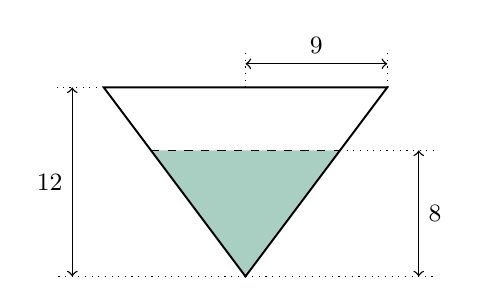
\begin{tikzpicture}[scale=0.2]
\fill[badge] (0,0)--(-6,8)--(6,8)--cycle;
\draw[line width=0.7pt] (-9,12)--(0,0)--(9,12)--cycle;
\draw[line width=0.5pt,dashed] (-6,8)--(6,8);
\draw[line width=0.4pt,dotted] (6,8)--(12,8); \draw[line width=0.4pt,dotted] (0,0)--(12,0);
\draw[line width=0.5pt,<->] (11,0)--(11,8);
\node[right,font=\small] at (11,4) {8};
\draw[line width=0.4pt,dotted] (-9,12)--(-12,12); \draw[line width=0.4pt,dotted] (0,0)--(-12,0);
\draw[line width=0.5pt,<->] (-11,0)--(-11,12);
\node[left,font=\small] at (-11,6) {12};
\draw[line width=0.4pt,dotted] (0,12)--(0,14.5); \draw[line width=0.4pt,dotted] (9,12)--(9,14.5);
\draw[line width=0.5pt,<->] (0,13.5)--(9,13.5);
\node[above,font=\small] at (4.5,13.5) {9};
\end{tikzpicture}}\par\vspace{2.2mm}
\hspace*{7mm}(A)\ $8$\\[1.8mm]
\hspace*{7mm}(B)\ $13.5$\\[1.8mm]
\hspace*{7mm}(C)\ $24$\\[1.8mm]
\hspace*{7mm}(D)\ $6$
\vfill}}
\end{textblock*}
\clearpage

% ===== Module 2, page 3 =====
\topicheader{8}{Mock Test 8}
\pagefooter{7}
\colrule{34}{236}
\mbox{}%
\pagekicker{Mock 8 \textperiodcentered{} Module 2 \textperiodcentered{} 22 questions \textperiodcentered{} 35 minutes}{Questions 17--22}
\begin{textblock*}{\COLW}(\LCOL,34mm)
{\fontsize{10.4}{13.4}\selectfont
\parbox[t][233mm][t]{\COLW}{%
\noindent\pnum{17} A bag holds 5 red tokens and $n$ blue tokens, where $n$ is a positive integer. Two tokens are drawn at random without replacement. The probability that the two tokens are the same color is $\frac{4}{9}$. What is the sum of all possible values of $n$?\par\vspace{2.2mm}
\hspace*{7mm}(A)\ $4$\\[1.8mm]
\hspace*{7mm}(B)\ $5$\\[1.8mm]
\hspace*{7mm}(C)\ $9$\\[1.8mm]
\hspace*{7mm}(D)\ $20$
\vfill

\noindent\pnum{18} If $\dfrac{1}{x}+\dfrac{6}{y}=4$ and $\dfrac{4}{x}-\dfrac{3}{y}=7$, what is the value of $x+y$?\gridbox
\vfill

\noindent\pnum{19} A club ran two training programs and recorded whether athletes improved their 5-kilometer time. The table shows, for each program and each kind of athlete, the number who improved out of the number who took part. Which of the following statements is supported by the table?\figwrap{\begin{tabular}{|l|c|c|}
\hline
 & Program A & Program B\\\hline
New & 9 of 10 & 160 of 200\\\hline
Experienced & 30 of 90 & 3 of 20\\\hline
\end{tabular}}\par\vspace{2.2mm}
\hspace*{7mm}(A)\ Program A had the higher improvement rate in each group, yet Program B's overall improvement rate was more than 30 percentage points higher.\\[1.8mm]
\hspace*{7mm}(B)\ Program A had the higher improvement rate in each group, and Program A's overall improvement rate was also higher.\\[1.8mm]
\hspace*{7mm}(C)\ Program B had the higher improvement rate in each group, and Program B's overall improvement rate was also higher.\\[1.8mm]
\hspace*{7mm}(D)\ Program A had the higher improvement rate in each group, yet Program B's overall improvement rate was less than 10 percentage points higher.
\vfill}}
\end{textblock*}
\begin{textblock*}{\COLW}(\RCOL,34mm)
{\fontsize{10.4}{13.4}\selectfont
\parbox[t][233mm][t]{\COLW}{%
\noindent\pnum{20} What is the sum of all integer values of $k$ for which the equation $x^{2}-2kx+k+12=0$ has no real solutions?\par\vspace{2.2mm}
\hspace*{7mm}(A)\ $6$\\[1.8mm]
\hspace*{7mm}(B)\ $4$\\[1.8mm]
\hspace*{7mm}(C)\ $0$\\[1.8mm]
\hspace*{7mm}(D)\ $3$
\vfill

\noindent\pnum{21} In the $xy$-plane, points $A(-1,2)$ and $B(7,k)$ are the endpoints of a diameter of a circle that is tangent to the $x$-axis. What is the value of $k$?\gridbox
\vfill

\noindent\pnum{22} The function $f$ is defined by $f(x)=x^{2}-6x+5$. What is the sum of all real solutions of the equation $f(f(x))=0$?\par\vspace{2.2mm}
\hspace*{7mm}(A)\ $6$\\[1.8mm]
\hspace*{7mm}(B)\ $12$\\[1.8mm]
\hspace*{7mm}(C)\ $4$\\[1.8mm]
\hspace*{7mm}(D)\ $18$
\vfill}}
\end{textblock*}
\clearpage

\end{document}
